\documentclass{beamer}

\usetheme{Darmstadt}

\usepackage{graphics,xcolor}
% \usepackage{stmaryrd,amssymb,amsmath}

\usepackage{docmute}
\usepackage{hyperref}
\newcommand{\nat}{\mathbb{N}}
\newcommand{\ints}{\mathbb{Z}}
\newcommand{\intersection}{\ensuremath{\cap}}
\newcommand{\emptyword}{\ensuremath{\epsilon}}
\newcommand{\len}[1]{\ensuremath{|#1|}}
\newcommand{\union}{\ensuremath{\cup}}
\newcommand{\deltahat}{\ensuremath{\widehat{\delta}}}
\title{2-way Deterministic Finite Automata}
\author{Balaji,Sannidhi,Sasmita,Ramanan}
\date{}
\institute{IISc Bangalore}
\begin{document}
\maketitle
\documentclass{beamer}
\usetheme{Darmstadt}
\usecolortheme{orchid}
\usepackage{tikz}
\usetikzlibrary{automata, positioning}
\usepackage{graphics,xcolor}

\newcommand{\nat}{\mathbb{N}}
\newcommand{\ints}{\mathbb{Z}}
\newcommand{\intersection}{\ensuremath{\cap}}
\newcommand{\emptyword}{\ensuremath{\epsilon}}
\newcommand{\len}[1]{\ensuremath{|#1|}}
\newcommand{\union}{\ensuremath{\cup}}
\newcommand{\deltahat}{\ensuremath{\widehat{\delta}}}

\title[Finite-State Automata]{2-way DFA}
\author{xyz}

\begin{document}

\begin{frame}
\frametitle{Outline}
\tableofcontents
\end{frame}

\section{Introduction}

\begin{frame}{What is 2DFA?}
  \begin{block}{2DFA}
    A Two-Way Deterministic Finite Automaton (2DFA) is a type of finite state machine that extends the capabilities of a regular Deterministic Finite Automaton (DFA) by allowing its read head to move \textcolor{red}{bidirectionally} along the input tape. 
   
    
  \end{block}
  \begin{itemize}
    \item 2DFAs were introduced in 1959 by Rabin and Scott.
   \end{itemize}

\end{frame}

\begin{frame}
\frametitle{How 2DFA works?}
%construction of tape to illustrate the working of 2DFA drawing 
\centering
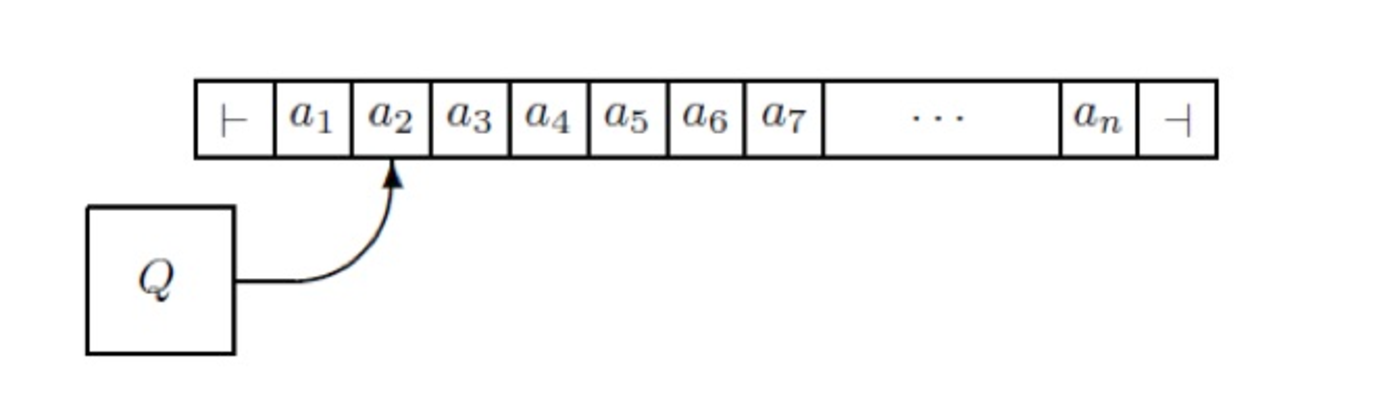
\includegraphics[width=0.65\textwidth]{Screenshot 2024-03-15 at 3.05.42 PM.pdf}
\begin{itemize}
  \item Two-way Finite Automata has a read head, which
can move left or right over the input string .
\item Read head can revisit the input symbols any number of times.
\item The input string is enclosed between left and right
endmarkers $\vdash$ and $\dashv$, which are not elements of the
input alphabet $\Sigma$.
\item The read head will not move outside of the
endmarkers.
\item A 2DFA needs only a single accept state and a single reject state.
\end{itemize}
\end{frame}

\begin{frame}{Turing Machine vs 2DFA}
  
    \textbf{Turing Machine:}
    \begin{itemize}
      \item Contains a \textcolor{violet}{read/write} head that moves left or right along the tape 
      \item Has \textcolor{violet}{unbounded} memory.
    \end{itemize}
    \hspace*{1cm}\\
    \textbf{2DFA:}
    \begin{itemize}
      \item Has  \textcolor{violet}{read} only head that moves left or right along the tape.
      \item Has \textcolor{violet}{finite} memeory like DFA.
    \end{itemize}
  
\end{frame}

\section{Formal Definitions, Notations and Construction}

\begin{frame}
\frametitle{Formal representation of 2DFA}

A \emph{2DFA} is of the form 
\textbf{\[(Q, \Sigma, \vdash, \dashv, \delta, s, t, r)\]}
where,
\begin{itemize}
\item $Q$ is a finite set of states.
\item $\Sigma$ is a finite set of input symbols.
\item $\vdash$ is the left endmarker. ($\vdash \notin \Sigma$)
\item $\dashv$ is the right endmarker. ($\dashv \notin \Sigma$)
\item $\delta : Q \times (\Sigma \cup \{\vdash, \dashv\}) \rightarrow Q \times \{L, R\}$ is a transition function. \\(L $=$ left, R $=$ right)
\item $s \in Q$ is the start state.
\item $t \in Q$ is the accept state.
\item $r \in Q$ is the reject state ($r \neq t$).
\end{itemize}
\end{frame}

\begin{frame}
\frametitle{Properties of transition function}

For all states $p$,
\begin{itemize}
\item \textcolor{red}{$\delta(p,\vdash) = (q,R)$}, for some $q \in Q$ 
\item \textcolor{red}{$\delta(p, \dashv) = (q, L)$}, for some $q \in Q $
\end{itemize}
\hspace*{1cm}\\
Current input symbol is $a \in \Sigma \cup \{\vdash\}$, $t =$ accept state, $r =$ reject state.
\begin{itemize}
\item \textcolor{red}{$\delta(t,a) = (t,R)$ and $\delta(t,\dashv) = (t,L)$} 
\item \textcolor{red}{$\delta(r,a) = (r,R)$ and $\delta(r,\dashv) = (r,L)$}
\end{itemize}
\hspace*{1cm}\\
 In general, $\delta(p,a) = (q,d)$ where $p,q \in Q$ and $d \in \{L,R\}$

\end{frame}

%\begin{frame}{Example 2DFA}
%\begin{exampleblock}{2DFA for $a^{*}$}
%\begin{tikzpicture}[shorten >=1pt,node distance=2.5cm,on grid,auto] 
%\node[state,initial] (q0) {$q_0$}; 
%\node[state,accepting] (q1) [right=of q0] {$q_1$};
%\node[state] (q2) [below=of q0] {$q_2$};
%\path[->] 
%(q0) edge [loop above] node {($a,R$),($\vdash, R$)} (q0)
 %       edge node {$\dashv,L$} (q1)
  %      edge node {$b,R$} (q2)
%(q1) edge [loop above] node {$a,R$} (q1)
 %        edge [loop right] node {$b,R$} (q1)
  %       edge [loop below] node {($\dashv,L$),($\vdash, R$)} (q1)
%(q2) edge [loop left] node {$a,R$} (q2)
 %        edge [loop below] node {$b,R$} (q2)
  %       edge [loop right] node {($\dashv,L$),($\vdash, R$)} (q2);
%\end{tikzpicture}
%\end{exampleblock}
%\end{frame}

\begin{frame}
\frametitle{Example 2DFA}
 \centering
        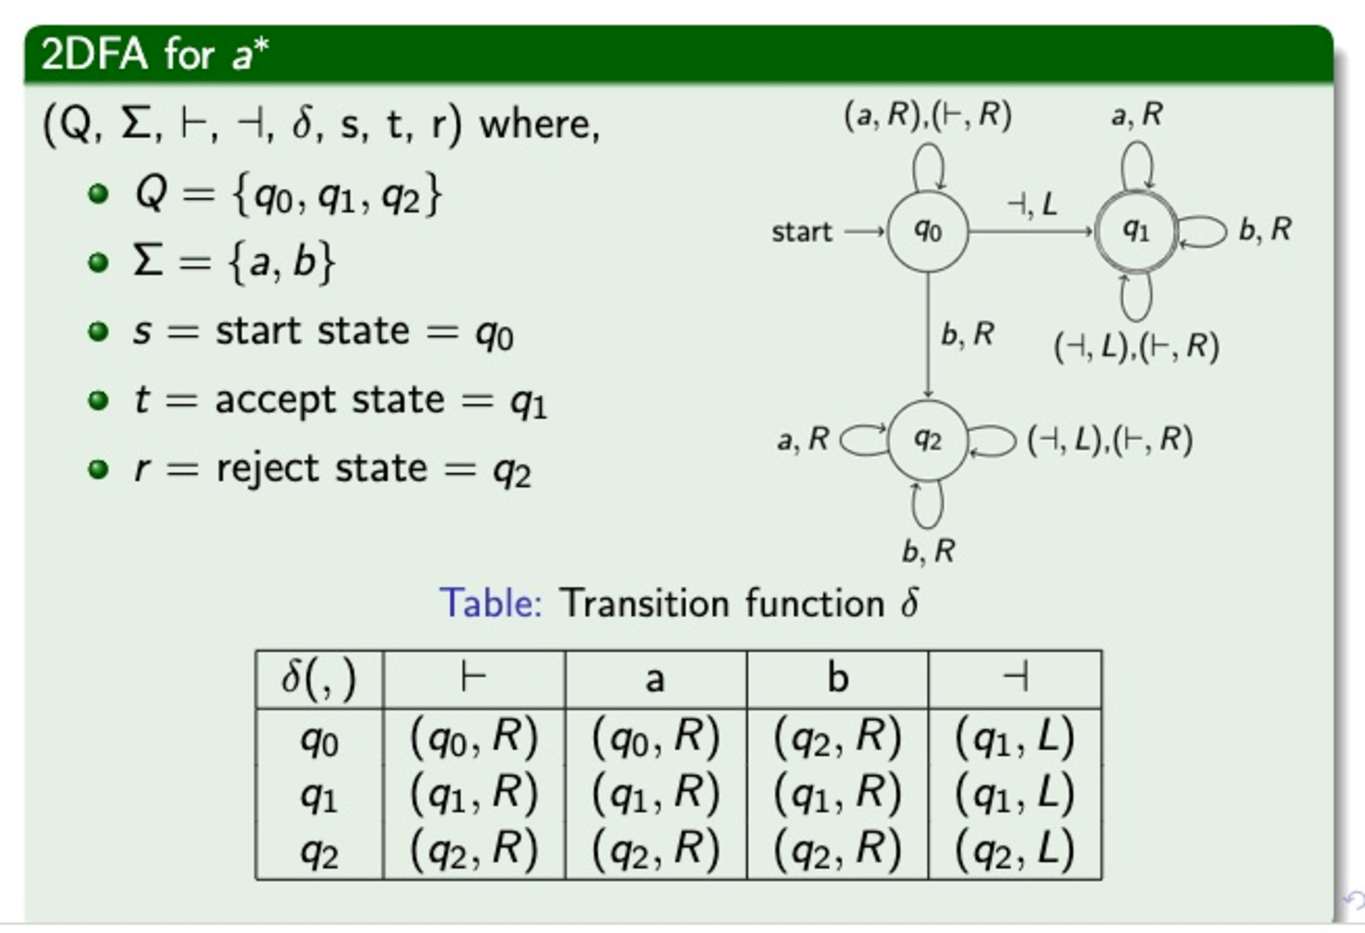
\includegraphics[width=1.0\textwidth]{Screenshot 2024-03-15 at 6.08.48 PM copy.pdf}
    
\end{frame}

\begin{frame}{Configurations }
Fix an input $x \in \Sigma^{*}$. $x = a_{1}a_{2}a_{3} \ldots a_{n}$. Let $a_{0} = \vdash$ and $a_{n+1} = \dashv$. \\
$a_0a_1a_2a_3 \ldots a_n a_{n+1} = \vdash x \dashv$. \\
\begin{block}{Configuration}
A configuration of the machine on input $x$ is a pair $(q, i)$ such that $q \in Q$ and $0 \leq i \leq n + 1$. Informally, the pair $(q, i)$ gives a \textcolor{red}{current state} and \textcolor{red}{current position} of the read head. \\
The \textcolor{red}{start configuration is $(s, 0)$}, meaning that the machine is in its start state $s$ and scanning the left endmarker.
\end{block}
A binary relation $\xrightarrow[x]{1}$, the next configuration relation, is defined on configurations as follows:
\[
\delta(p, a_i) = (q, L) \Rightarrow (p, i) \xrightarrow[x]{1} (q, i - 1),
\]
\[
\delta(p, a_i) = (q, R) \Rightarrow (p, i) \xrightarrow[x]{1} (q, i + 1).
\]
\end{frame}

\begin{frame}{Configurations }
The relation $\xrightarrow[x]{1}$ describes one step of the machine on input $x$. We define the relations $\xrightarrow[x]{n}$ inductively, $n \geq 0$:
\begin{itemize}
\item $(p, i) \xrightarrow[x]{0} (p, i)$
\item if $(p, i) \xrightarrow[x]{n}(q, j)$ and $(q, j) \xrightarrow[x]{1} (u, k)$, then $(p, i) \xrightarrow[x]{n+1} (u, k)$.
\end{itemize}
\hspace*{1cm}\\
For any configuration $(p, i)$, there is exactly one configuration $(q, j)$ such that $(p, i) \xrightarrow[x]{n} (q, j)$. \\


\end{frame}
\begin{frame}{Acceptance and Rejection}
  
    \hspace*{1cm}$(p,i) \xrightarrow[x]{*} (q,j)$ iff  $\exists$$n \geq 0$ such that $(p,i) \xrightarrow[x]{n} (q,j)$.
    
\begin{block}{Acceptance}
The input $x$ is accepted by the machine iff $(s, 0) \xrightarrow[x]{*} (t, k)$ for some k.
\end{block}
\begin{block}{Rejection}
  \begin{itemize}
\item The input $x$ is rejected by the machine if $(s, 0) \xrightarrow[x]{*} (r, k)$ for some k.
\end{itemize}
\end{block}

  
 If the machine neither reaches accept state nor reject state then the machine is said to be looping on that input.\\
 
Language accepted by the machine = $\{x \in \Sigma^{*} | x$ is accepted by the machine$\}$.

  \end{frame}


\begin{frame}{Constructing 2DFA 'M'}
  %length of a is divisible by 3 and length of b is divisible by 2
   $L(M) = \{x \in \Sigma^* \mid \#a(x)$ is multiple of 3, $\#b(x)$ is multiple of 2\}
  \begin{exampleblock}{Machine Description}
  \begin{itemize}
  \item Machine starts scanning from the left endmarker.
  \item Scan input string from left to right, counting only 'a's. If the count of 'a's is not a multiple of 3, reject and enter state $r$.\\
  \item Let $q_0,q_1,q_2$ be the states for counting 'a's. \\$q_0$: 3k; $q_1$: 3k+1; $q_2$: 3k+2.
  \item If the count of 'a's is a multiple of 3, start scanning from the right, counting only 'b's. If the count of 'b's is not a multiple of 2, enter state $t$; otherwise, enter state $r$.\\
  \item Let $p_0,p_1$ be the states for counting 'b's. \\$p_0$: 2k; $p_1$: 2k+1.
  \end{itemize}
  \end{exampleblock}
\end{frame}

\begin{frame}{Constructing 2DFA 'M'}
  %to check for few inputs and their acceptance 1.abba 2.bbaabab
  \centering
  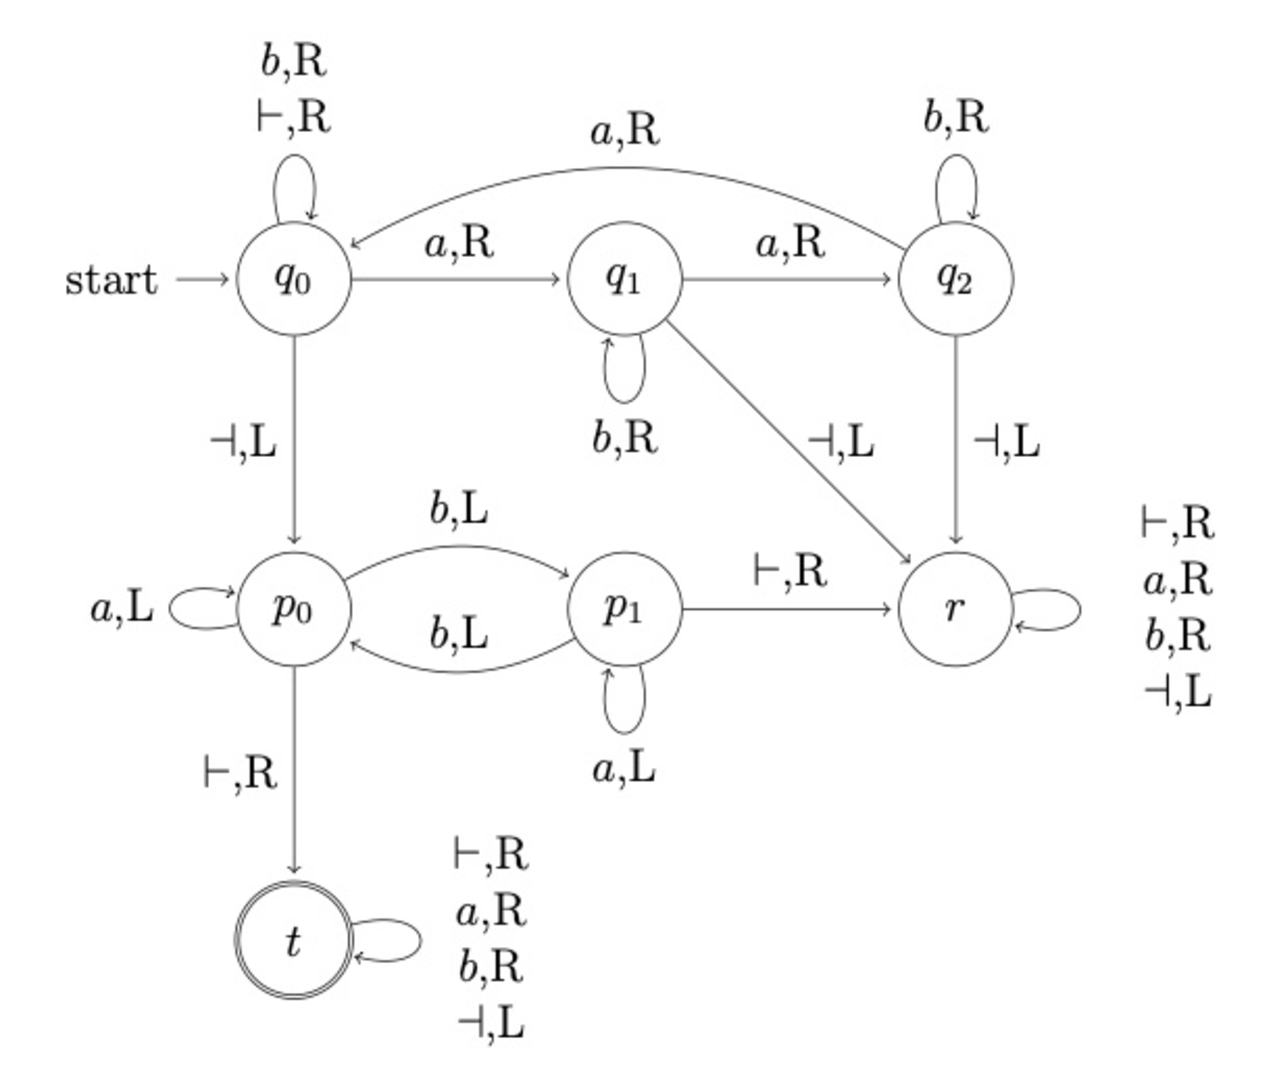
\includegraphics[width=0.6\textwidth]{Screenshot 2024-03-13 at 3.50.28 PM.pdf}
  \begin{itemize}
    
    \item input $=$ bbaabab :\\
    
       $ q_0 \xrightarrow{\vdash} q_0 \xrightarrow{b} q_0 \xrightarrow{b} q_0 \xrightarrow{a} q_1 \xrightarrow{a} q_2 \xrightarrow{b} q_2 \xrightarrow{a} q_0 \xrightarrow{b} q_0 \xrightarrow{\dashv} p_0 \xrightarrow{b} p_1 \xrightarrow {a} p_1 \xrightarrow{b} p_0 .....\xrightarrow{\dashv} t$\\
     
  \end{itemize}
\end{frame}

  \section{Languages accepted by 2DFA}
\begin{frame}{DFA to 2DFA conversion}
\begin{block}{Theorem}
  \begin{itemize}
  \item 2DFA only accepts regular languages.\\
  \item L(2DFA) = L(DFA) = Regular languages\\ 
  \end{itemize}
\end{block}

\begin{block}{Proof: L(DFA) $\subseteq$ L(2DFA)}
  For an arbitary DFA 'X', let us construct a 2DFA 'Y' that accepts the same language as X.\\
  
\begin{itemize}
  \item X : (Q, $\Sigma$, $\delta$, s, F)\\
  \item Let Y : (Q $\cup$ \{t, r\}, $\Sigma$, $\vdash$, $\dashv$, $\delta'$, s, t, r)\\
  %delta is defined as delta union transition from (final start in F , left end marker) to (t, L) and  (non final start i.e  Q-F , left end marker) to (r, L) and (s, right end marker ) to (s,R)
  \item $\delta'$: $\delta_R$ $\cup $ {\\
$\delta'$((s, $\vdash$)) = (s, R)\\
  $\delta'$((f, $\dashv$)) = (t, L) for f $\in$ F ;\hspace*{0.1cm} $\delta'$((n, $\dashv$)) = (r, L) for n $\in$ Q-F.\\
   $\delta'$((t, a)) = (t, R) ;\hspace*{0.3cm} $\delta'$((r, a)) = (r, R) for a $\in$ $\Sigma-\{\dashv\}$ }\\
   $\delta'$((t,$\dashv))$ = (t,L) ;\hspace*{0.5cm} $\delta'$((r,$\dashv))$ = (r,L)\\
    \end{itemize}
\end{block}
 
\end{frame}

\begin{frame}{DFA to 2DFA conversion}
  \begin{block}{Proof: L(X) $\subseteq$ L(Y)}
  \begin{itemize}
    \item Let x $\in$ L(X), len(x)=n. \\
    \item Then, $\deltahat$(s,x) = f where f $\in$ F \\
    \item (s,0) $\xrightarrow[\vdash x \dashv]{1}$ (s,1) $\xrightarrow[\vdash x \dashv]{n}$ (f,n+1) $\xrightarrow[\vdash x \dashv]{1}$ (t,n) .\\
    \item As (s,0) $\xrightarrow[\vdash x \dashv]{*}$ (t,n+1), x $\in$ L(Y).\\
    \item Hence, L(X) $\subseteq$ L(Y).\\
  \end{itemize}
  \end{block}
  Recall: \\
  A configuration of the machine on input $x$ is the pair \textcolor{blue}{$(q, i)$} , which gives the \textcolor{blue}{current state} and \textcolor{blue}{current position of the read head}. \\
  $(s, 0)$ means that the machine is in its start state $s$ and scanning the left endmarker.
  
\end{frame}

\begin{frame}{DFA to 2DFA conversion}
  \begin{block}{Proof: L(Y) $\subseteq$ L(X)}
  \begin{itemize}
    \item Let x $\in$ L(Y), len(x)=n. \\
    \item Then (s,0) $\xrightarrow[\vdash x \dashv]{*}$ (t,m) in Y\\
    \item So (s,0) $\xrightarrow[\vdash x \dashv]{1}$ (s,1) $\xrightarrow[\vdash x \dashv]{n}$ (f,n+1) $\xrightarrow[\vdash x \dashv]{1}$ (t,n) .\\
    \item As $\deltahat$(s,x) = f where f $\in$ F, x $\in$ L(X)\\
    
    \item Hence, L(Y) $\subseteq$ L(X).\\
  \end{itemize}
  \end{block}
   \textbf{Therefore, L(Y) = L(X)}
\end{frame}


\end{document}

\documentclass{beamer}
\usetheme{Darmstadt}
\usepackage{amssymb}
\usepackage{graphicx}

\newcommand{\nat}{\mathbb{N}}
\newcommand{\ints}{\mathbb{Z}}
\newcommand{\intersection}{\ensuremath{\cap}}
\newcommand{\emptyword}{\ensuremath{\epsilon}}
\newcommand{\len}[1]{\ensuremath{|#1|}}
\newcommand{\union}{\ensuremath{\cup}}

\title{Introduction to Automata Theory}
\author{Sannidhi}
\institute{IISc Bangalore}

\begin{document}



\begin{frame}
\frametitle{Language accepted by a 2-way DFA is regular}
\begin{itemize}
\item Claim: The language accepted by a 2-way finite automaton is regular
\item We will prove this using Myhill-Nerode theorem
\item Recall that the Myhill-Nerode theorem states that a language is regular if and only if the canonical equivalence relation has finitely many equivalence classes
\end{itemize}
\end{frame}

\begin{frame}
\frametitle{Language accepted by a 2-way DFA is regular}
\begin{itemize}
\item Let $M = (Q, \Sigma, \vdash, \dashv, \delta, s, t, r)$ be a 2-way finite automaton
\item Let $w = xz$ be a string in $\Sigma^*$
\item As the automaton is 2-way, its read head can cross the boundary between $x$ and $z$ several times.
\item Consider the function $T_x : (Q\cup\{\bullet\}) \rightarrow (Q\cup\{\bot\})$
\item If the automaton goes to state $q$ when it first crosses the boundary between $x$ and $z$, define $T_x(\bullet) = q$
\item If the read head never crosses the boundary between $x$ and $z$, define $T_x(\bullet) = \bot$
\end{itemize}
\end{frame}

\begin{frame}
\frametitle{Language accepted by a 2-way DFA is regular}
\begin{itemize}
\item Suppose the read head comes back from $z$ to $x$ and reaches state $q$
\item Then it may either go back to $z$ reaching state $p$, in which case define $T_x(q) = p$
\item Else, it may never go back to $z$, in which case define $T_x(q) = \bot$
\item Note that the function $T_x$ is well-defined as the automaton is deterministic
\item Also, $T_x$ depends only on $x$ and is independent of $z$
\item And if $y$ is another string in $\Sigma^*$ such that $T_x = T_y$, then $yz$ is accepted by the automaton if and only if $xz$ is accepted by the automaton
\end{itemize}
\end{frame}

\begin{frame}
\frametitle{Language accepted by a 2-way DFA is regular}
\begin{itemize}
\item Hence, $xRy$ if and only if $T_x = T_y$ becomes a canonical equivalence relation
\item Since the number of unique functions is finite (at most $(k+1)^{k+1}$), the canonical equivalence relation has finitely many equivalence classes
\item Hence the language accepted by the 2-way DFA is regular
\end{itemize}
\end{frame}

\begin{frame}
\frametitle{Example}
\begin{itemize}
\item Let us consider an example of a 2-way DFA accepting the language $L = \{x\in\{a,b\}^* | \#a(x) \text{ is a multiple of 3 and } \#b(x) \text{ is even}\}$
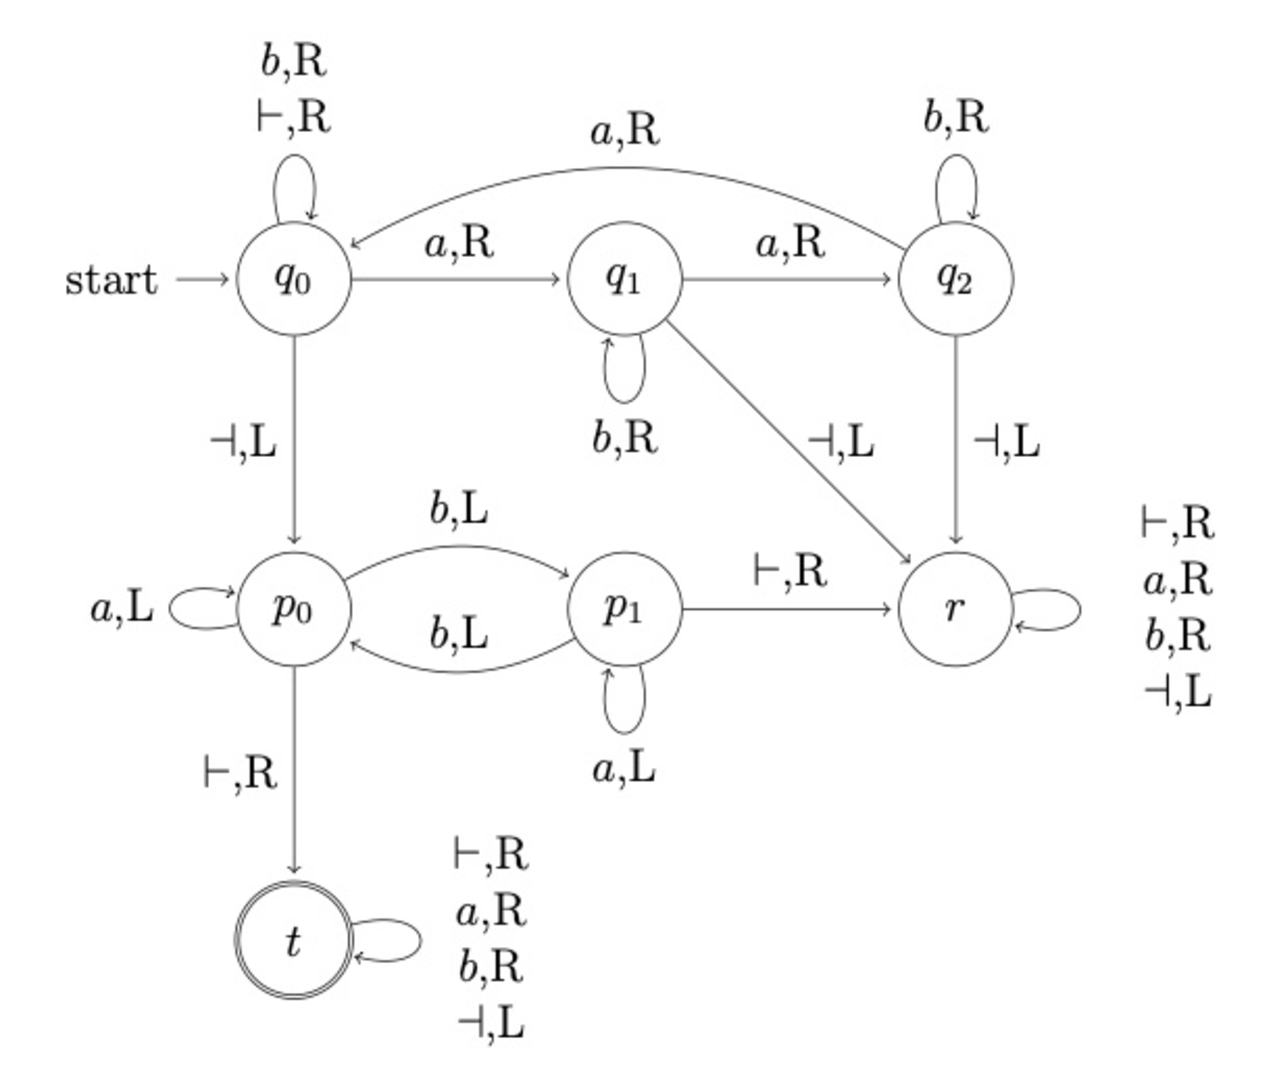
\includegraphics[width=0.6\textwidth]{dfa4.pdf}
\end{itemize}
\end{frame}

\begin{frame}
\frametitle{Example}
\begin{itemize}
\item For any $x\in\{a,b\}^*$,
\item If $\#a(x) = k \mod 3$, then $T_x(\bullet) = p_k$
\item If $\#b(x) = 0 \mod 2$, then $T_x(p_0) = t$ and $T_x(p_1) = r$
\item If $\#b(x) = 1 \mod 2$, then $T_x(p_0) = r$ and $T_x(p_1) = t$
\item And $T_x(t) = t$, $T_x(r) = r$
\item Hence, the canonical equivalence relation has 6 equivalence classes and the language is regular
\end{itemize}
\end{frame}

\begin{frame}
\frametitle{Constructing DFA from 2-way DFA}
\begin{itemize}
\item Once we have the canonical equivalence relation, we can easily construct a DFA.
\item Let $M = (Q, \Sigma, \vdash, \dashv, \delta, s, t, r)$ be a 2-way finite automaton
\item Let $Q'$ be the set of all equivalence classes of the canonical equivalence relation
\item $s' = T_{\emptyword}$
\item $\delta'(T_x, a) = T_xa$
\item $F' = \{T_x|x\in L(M)\}$
\item DFA $M' = (Q', \delta', s', F')$ will accept the same language as the 2-way DFA $M$
\end{itemize}
\end{frame}

\begin{frame}
\frametitle{Example}
\begin{itemize}
\item The DFA accepting the same language as the 2-way DFA is as follows:
\end{itemize}
\begin{figure}
    \centering
        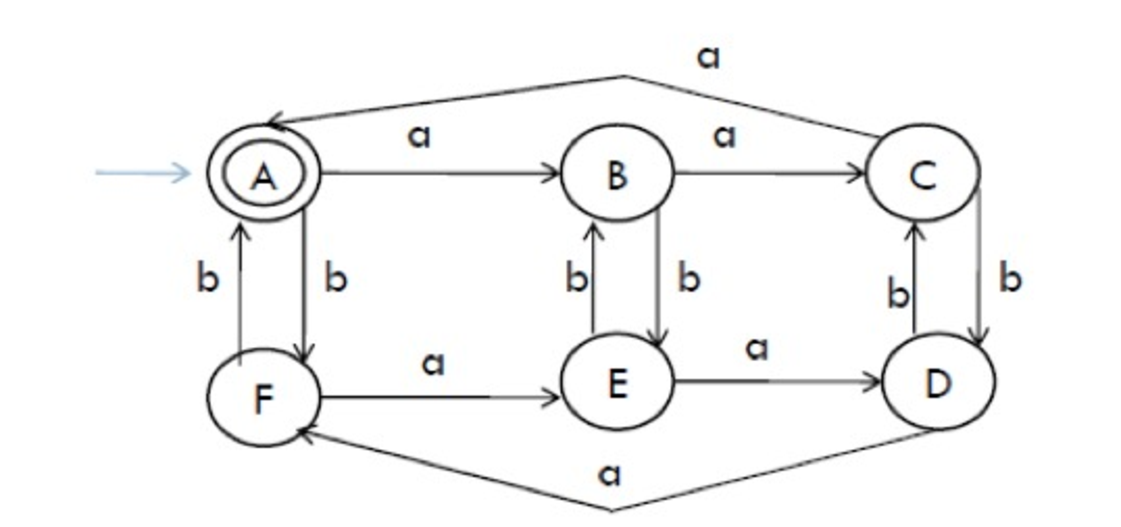
\includegraphics[width=0.6\textwidth]{dfa5.pdf}
\end{figure} 
\end{frame}

\end{document}

\documentclass{beamer}

\usetheme{Darmstadt}

\usepackage{graphics,xcolor}
\usepackage{graphicx}

% \usepackage{stmaryrd,amssymb,amsmath}

\newcommand{\nat}{\mathbb{N}}
\newcommand{\ints}{\mathbb{Z}}
\newcommand{\intersection}{\ensuremath{\cap}}
\newcommand {\emptyword}{\ensuremath{\epsilon}}
\newcommand {\len}[1] {\ensuremath{|#1|}}
\newcommand {\union} {\ensuremath{\cup}}



\begin{document}

\section{Established Results}



\begin{frame}
\frametitle{Unary finite automata}
Below, H(n) represents the function  $e^{\sqrt{nlog(n)}}$\\
\medskip
These are some statements related to unary finite automata
\medskip


\begin{itemize}
\item Each unary n-state 2dfa can be simulated by a 1dfa with O(H(n)) states.
\item For each n there is a unary n-state 2dfa A such that each 1dfa recognizing L(A) requires $\Omega$(H(n)) states.
\end{itemize}

\end{frame}




\begin{frame}
\frametitle{Unary finite automata}

 
\begin{itemize}
\item
For each n there is a unary n-state 2dfa A such that each 1nfa recognizing L(A) requires $\Omega$(H(n))
\item
Each unary n-state 1nfa A can be simulated by a 2dfa B with O($n^2$) states.
\item
For each n there is a unary n-state 1nfa A such that each 2dfa recognizing L(A) requires $\Omega$($n^2)$ states.
\end{itemize}

\end{frame}
\begin{frame}
\frametitle{Unary finite automata}
Informally speaking we can see that 2dfa's are hard to simulate by ldfa's, even if we consider only unary languages.\\
\medskip
Also, for unary languages,two-way motion is more powerful, in a sense, because we can simulate unary lnfa's by 2dfa's increasing the number of states only polynomially, which is not possible the other way round. 
\end{frame}
\begin{frame}
\frametitle{Unary finite automata}
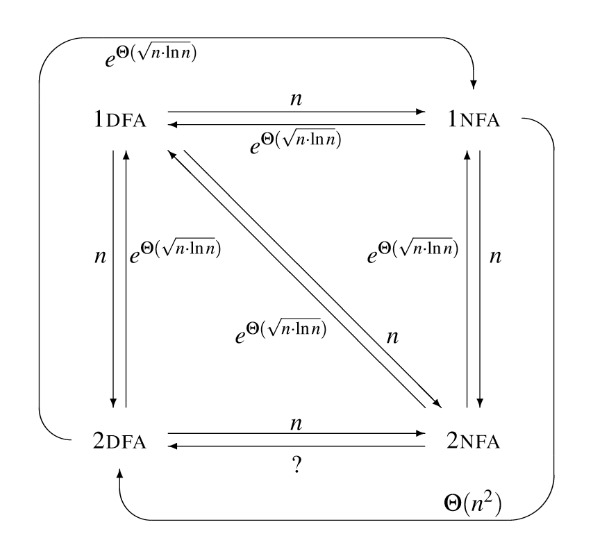
\includegraphics[width = 200 pt]{x}
\end{frame}
\begin{frame}
\frametitle{1nfa to 2dfa}
Lemma A: If gcd(a,b)=1, then the greatest number such that the equation $ax+by=c$ has no solutions in natural numbers is (a-1)(b-1)-1.\\
\medskip
Theorem:For each n there is a unary n-state 1nfa A such that each 2dfa recognizing L(A) requires $\Omega(n^2)$ states.\\
\medskip
Proof: Let L=$\{x| x= n x_1$+(n-1)$x_2$ for $x_1$, $x_2\in$N\}. L can be recognized by a lnfa
A with n states. A=(Q, $q_0$, E, F) is defined as follows: Q={$q_0$,..., $q_{n-l}$}, E =
\{($q_i$, $q_{i+1}$)$| i = 0,..., n- 1\}\cup {(q_1, q_3)}$ (the addition is mod n) and F = {$q_0$}. Let
m = max($\mathbb{N}$-L). By Lemma A, m = O($n^2$). Consider a 2dfa B recognizing L and its
computation on m. Suppose that, in all passes on m, B enters a cycle and let
$y_1$,...,$y_k$ be the lengths of these cycles. Then B would reject also m'=
m + lcm($y_1,.. , y_k$), which contradicts the fact that m' $\in$ L. Therefore, there is a pass.
of B on m without a cycle and the theorem follows. 

\end{frame}
\end{document}

\begin{frame}
\frametitle{(Unary)2-DFA to 1-NFA/1-DFA - A worst case example}
\begin{itemize}
    \item Let $F(n)$ be defined as follows:
    \item Maximum value of $lcm(x_1,x_2,\ldots x_k)$ such that $x_1+x_2+\ldots+x_k=n$ and $x_1,x_2,\ldots x_k \in \nat$
\end{itemize}

    Some properties of $F(n)$:
    \begin{itemize}
        \item $x_1,x_2,\ldots x_k$ can be found to be coprime satisfying $lcm(x_1,x_2\ldots x_k$)$ = F(n)$
        \item $F(n) = O(H(n))$\\
    \end{itemize}
\end{frame}
\begin{frame}   
    \frametitle{(Unary)2-DFA to 1-NFA/1-DFA - A worst case example}
    \begin{itemize}
        \item Let the language $L = \{a^{iF(n)} \mid i \in \nat\ , i \ge 1\}$.
        \item Take any 1-NFA accepting this language.
        \item Any simple path from a start state to a final state must have length at least $F(n)$.
        \item Canonical MN Relation has atleast $F(n)$ classes.
        \item But 2-DFA can do better. Have $x_i$ states to check divisibility by $x_i$.
        \item Upon seeing right end marker transition to new set of $x_{i+1}$ states if divisible by $x_i$. 
        \item Reject if not divisible by any $x_i$. Go to final state if divisible by all $x_i$. Total number of states = $n+2$.
    \end{itemize}
\end{frame}

\begin{frame}
    \frametitle{(Unary)2-DFA to 1-DFA - Best known Bound}
    \begin{itemize}
        \item Any unary 2-DFA with can be converted to 1-DFA with at most $O(H(n))$ states.
        \item Any 2-DFA can be converted into an equivalent sweeping 2-DFA without changing the number of states. [Chrobak]
        \item For accepting words of length $\le n$ accepted by the 2-DFA, we have n states, mark them as final accordingly
        \item Note that any word of length longer than n accepted by the 2-DFA must pass through a cycle/pump.
        \item Any given state can be a part of at most one of these cycles.
        \item Say on a word u of length more than n the machine passes through at most k cycles.
        
    \end{itemize}

\end{frame}
\begin{frame}
    \frametitle{(Unary)2-DFA to 1-DFA - Best known Bound}
    \begin{itemize}
        \item Let the lengths of the cycles be $y_1,y_2,\ldots y_k$. Then $y_1+y_2+\ldots y_k \le n$.
        \item If a machine accepts a word u of length more than n, it must also accept a word of length $|u| + lcm(y_1,y_2,\ldots y_k)$.
        \item Construct a 1-DFA with first n states as mentioned and a loop of length $lcm(y_1,y_2,\ldots y_k)$ attached to the last state. Mark states as final accordingly.
        \item Prove: This accepts the same language as the 2-DFA.
        \item The number of states in the 1-DFA is at most $n + lcm(y_1,y_2,\ldots y_k) \le n + F(n) = O(H(n))$.
    \end{itemize}
\end{frame}



\begin{frame}
    \frametitle{Some other automata}
    \begin{itemize}
        \item \textbf{2 way Non-deterministic Finite Automata:-} A two-way nondeterministic finite automaton (2NFA) may have multiple transitions defined in the same configuration.
        \item Its transition function is $\delta:(Q \times \Sigma\cup \{L,R\}) \rightarrow 2^{Q\times \{left,right\}}$
        \item A 2NFA accepts a string if at least one of the possible computations is accepting. Like the 2DFAs, the 2NFAs also accept only regular languages. 
        \item \textbf{Sweeping Automata:-} A two-way automaton performing head reversal only when the input head is visiting the endmarkers is
        called sweeping automaton.
        \item \textbf{Rotating Automata:-}A computation of a rotating automaton is a sequence of left-to-right scans of the input. In particular, when
        the right end of the input is reached, the computation continues on the leftmost input symbol. 
        
        
    \end{itemize}
\end{frame}
\begin{frame}
    \frametitle{Some other automata}
    \begin{itemize}
        \item In other words, we can imagine the input tape as circular, with a special cell containing a marker and connecting
        the end with the beginning of the tape.
        \item With a trivial transformation which doubles the number of the
        states, each rotating automaton can be transformed into an equivalent sweeping automaton.
        \item \textbf{2 way Alternating Finite Automata(AFA):} Structure same as 2 way NFA. Transitions divided into 2: existential and universal.
        \item Existential and universal transitions simulate all possible moves that can be made. Every state is given a truth value.
        \item Even if there is one simulation that leads to a final state, existential transitions return 1. Universal transitions return 1 only if all simulations lead to a final state.
        
    \end{itemize}
\end{frame}
\begin{frame}
    \frametitle{Other established results and open problems}
    \begin{itemize}
        \item Christos Kapoutsis determined that transforming an $n$-state 2-DFA to an equivalent 1-DFA requires $ {\displaystyle n(n^{n}-(n-1)^{n})}$ states in the worst case.
        \item If an $n$-state 2DFA or a 2NFA is transformed to a 1-NFA, the worst-case number of states required is $ {2n \choose n+1}= O ( \frac{4 ^n}{ \sqrt{n}} ) $.
        \item Sipser constructed a sequence of languages, each accepted by an n-state NFA, yet which is not accepted by any sweeping automata with fewer than $ {\displaystyle 2^{n}}$ states. 
        \item \textbf{Sakoda-Sipser's open problem:-} Is there a 2-DFA with polynomial number of states accepting the same language as a 2-NFA?  
        \item \textbf{Another open problem:} What is the relationship between unary 1-afa's (or 2-afa's) and other fa's? It
        is easy to show some lower and upper bounds for 1-afa's with only universal states.
    \end{itemize}
\end{frame}
\begin{frame}
    \frametitle{References}
    \begin{itemize}
       \item Papers referenced are available on  \href{https://github.com/blackscreen-whitetext/Automata_Seminar}{\textcolor{blue}{Github}}
       \item \href{https://en.wikipedia.org/wiki/Two-way_finite_automaton}{\textcolor{blue}{Wikipedia link}}
    \end{itemize}
\end{frame}
\end{document}